% =====================================================================
%  fuel_cell_types.tex  --  the three partially loaded fuel-cell variants that
%  occur in the core, drawn like the fuel-cell square of Figure~\ref{fig:fuelcell}
%  but with no dimensions or labels.  Left: half-filled (only the top two rod rows
%  loaded); middle: middle-empty (inner 2x2 unloaded); right: corner-empty (the
%  top-left corner triangle unloaded).  The omitted lattice positions stay water
%  (yellow).  Three cells side by side; the coordinate unit (0.524 cm = 80%% of
%  the earlier 0.655 cm) sets the total width to ~0.76 of the 16 cm text width --
%  NOT \resizebox.
%  \input from chapters/2-geometry.tex.
% =====================================================================
\newcommand{\fctypebase}{%
  \fill[yellow]          (-3.6,-3.6)   rectangle (3.6,3.6);    % water (cell)
  \fill[green!75!black]  (-3.4,-3.4)   rectangle (3.4,3.4);    % Al box wall
  \fill[yellow]          (-3.25,-3.25) rectangle (3.25,3.25);  % water cavity
  \foreach \g in {-1.625,0,1.625}{
    \draw[thin] (\g,-3.25) -- (\g,3.25);
    \draw[thin] (-3.25,\g) -- (3.25,\g);}
  \draw[thick] (-3.6,-3.6)   rectangle (3.6,3.6);
  \draw        (-3.4,-3.4)   rectangle (3.4,3.4);
  \draw        (-3.25,-3.25) rectangle (3.25,3.25);}
\begin{figure}[H]
  \centering
  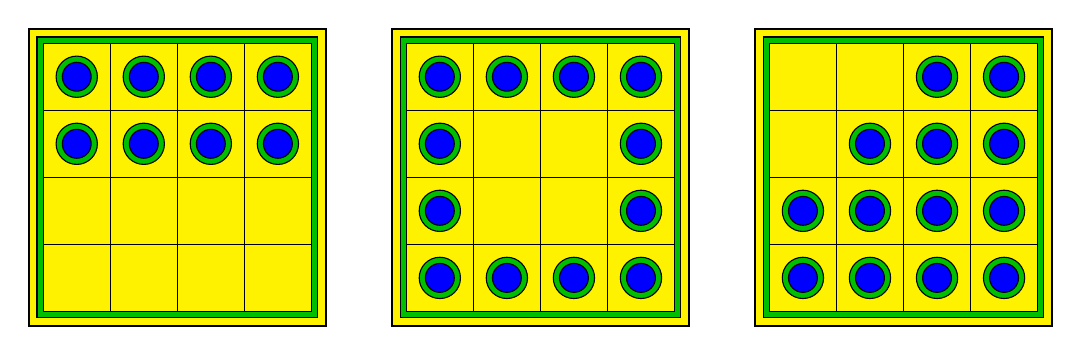
\begin{tikzpicture}[x=0.524cm,y=0.524cm]
    % ---- left: half-filled (top two rod rows only) ----
    \begin{scope}[shift={(0,0)}]
      \fctypebase
      \foreach \x/\y in {%
        -2.4375/2.4375,-0.8125/2.4375,0.8125/2.4375,2.4375/2.4375,%
        -2.4375/0.8125,-0.8125/0.8125,0.8125/0.8125,2.4375/0.8125}{
          \fill[green!75!black] (\x,\y) circle (0.5);
          \draw[thin]           (\x,\y) circle (0.5);
          \fill[blue]           (\x,\y) circle (0.35);
          \draw[thin]           (\x,\y) circle (0.35);}
    \end{scope}
    % ---- middle: middle-empty (inner 2x2 unloaded) ----
    \begin{scope}[shift={(8.8,0)}]
      \fctypebase
      \foreach \x/\y in {%
        -2.4375/2.4375,-0.8125/2.4375,0.8125/2.4375,2.4375/2.4375,%
        -2.4375/0.8125,2.4375/0.8125,%
        -2.4375/-0.8125,2.4375/-0.8125,%
        -2.4375/-2.4375,-0.8125/-2.4375,0.8125/-2.4375,2.4375/-2.4375}{
          \fill[green!75!black] (\x,\y) circle (0.5);
          \draw[thin]           (\x,\y) circle (0.5);
          \fill[blue]           (\x,\y) circle (0.35);
          \draw[thin]           (\x,\y) circle (0.35);}
    \end{scope}
    % ---- right: corner-empty (top-left corner triangle unloaded) ----
    \begin{scope}[shift={(17.6,0)}]
      \fctypebase
      \foreach \x/\y in {%
        0.8125/2.4375,2.4375/2.4375,%
        -0.8125/0.8125,0.8125/0.8125,2.4375/0.8125,%
        -2.4375/-0.8125,-0.8125/-0.8125,0.8125/-0.8125,2.4375/-0.8125,%
        -2.4375/-2.4375,-0.8125/-2.4375,0.8125/-2.4375,2.4375/-2.4375}{
          \fill[green!75!black] (\x,\y) circle (0.5);
          \draw[thin]           (\x,\y) circle (0.5);
          \fill[blue]           (\x,\y) circle (0.35);
          \draw[thin]           (\x,\y) circle (0.35);}
    \end{scope}
  \end{tikzpicture}
  \caption{The three partially loaded fuel-cell variants.}
  \label{fig:fuelcelltypes}
\end{figure}
